\part{A Multi-Agent System for Optimization}

\chapter{Agent-Based Modeling of an Optimization Problem}

\section{Problem Modeling with NDMO}\label{modeling}

In answer to the previous shortcomings, we propose a generic approach called Natural Domain Modeling for Optimization (NDMO) that relies on a natural or intrinsic description of the problem (\textit{i.e.} close to the reality being described).

\begin{figure}[]
	\centering
	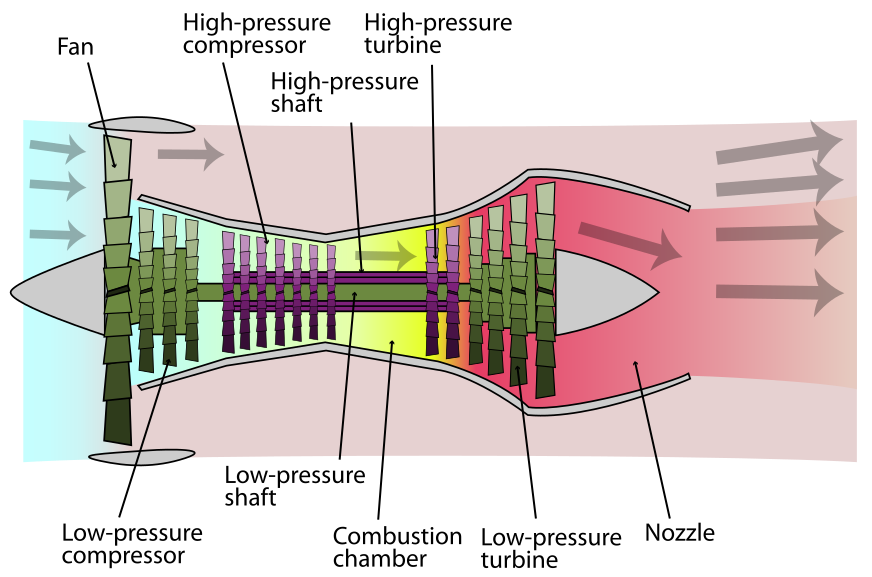
\includegraphics[width=0.8\textwidth]{Turbofan_operation}
	\caption{Illustration of a Turbofan engine (CC SA-BY  \href{http://en.wikipedia.org/wiki/File:Turbofan_operation.svg}{K. Aainsqatsi})}
	\label{turbofan_illu}
\end{figure}

To illustrate how an optimization problem is modeled, we use a simplified Turbofan optimization problem. On \figurename{} \ref{turbofan_illu}, an illustration of the principle of the turbofan can be seen. In this figure, the bypass ratio is the ratio between the air drawn in by the fan not entering engine core (which is \emph{bypassed}) and the air effectively used for the combustion process. The pressure ratio is the ratio between pressure produced by the compressors and the pressure it receives from the environment.

In order to identify the elements of a generic continuous optimization model, we worked with experts from several related fields: numerical optimization, mechanics as well as aeronautics and engine engineers. As a result, we identified five classes of interacting entities: \emph{models}, \emph{design variables}, \emph{output variables}, \emph{constraints} and \emph{objectives}. These entities and their relations are represented by the diagram in \figurename{} \ref{class_diag}, that we detail next.

\begin{figure}[t]
	\centering
	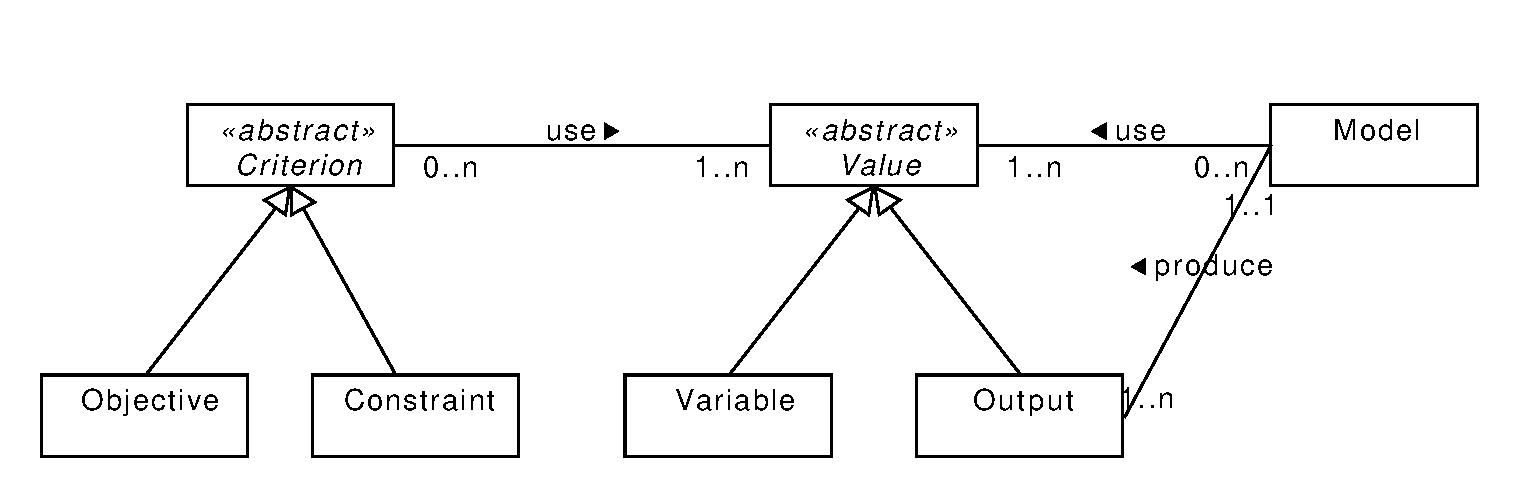
\includegraphics[width=0.9\textwidth]{class_diag}
	\caption{Class diagram of MDO problems}
	\label{class_diag}
\end{figure}

In \figurename{} \ref{turbofan:math}, the analytic expression of this optimization problem is given, while in \figurename{} \ref{turbofan:graph}, the problem is presented as a graph of the different entities. The design variables of this problem are $pi\_c$ and $bpr$, which indicate respectively the compressor pressure ratio and the bypass ratio of the engine. The turbofan model produces three outputs: $Tdm0$, $s$ and $fr$, representing respectively the thrust, fuel consumption and thrust ratio of the engine. In this problem we try to maximize the thrust and minimizing the fuel consumption while satisfying some feasibility constraints. 

\begin{figure}[]
\centering
\subfloat[mathematical formulation.]{\begin{minipage}{0.4\textwidth}
		$\begin{array}{c}
			(Tdm0, s, fr) = Turbofan(pi\_c, bpr) \\
			max \; Tdm0 \\
			min \; s \\
			subject \; to \\
			s \leq 155 \\
			fr \geq 4
		\end{array}$
\label{turbofan:math}
\end{minipage}}\hfill%
\subfloat[{corresponding entities graph.}]{\begin{minipage}{0.6\textwidth}%
		\centering
		\label{turbofan:graph}
		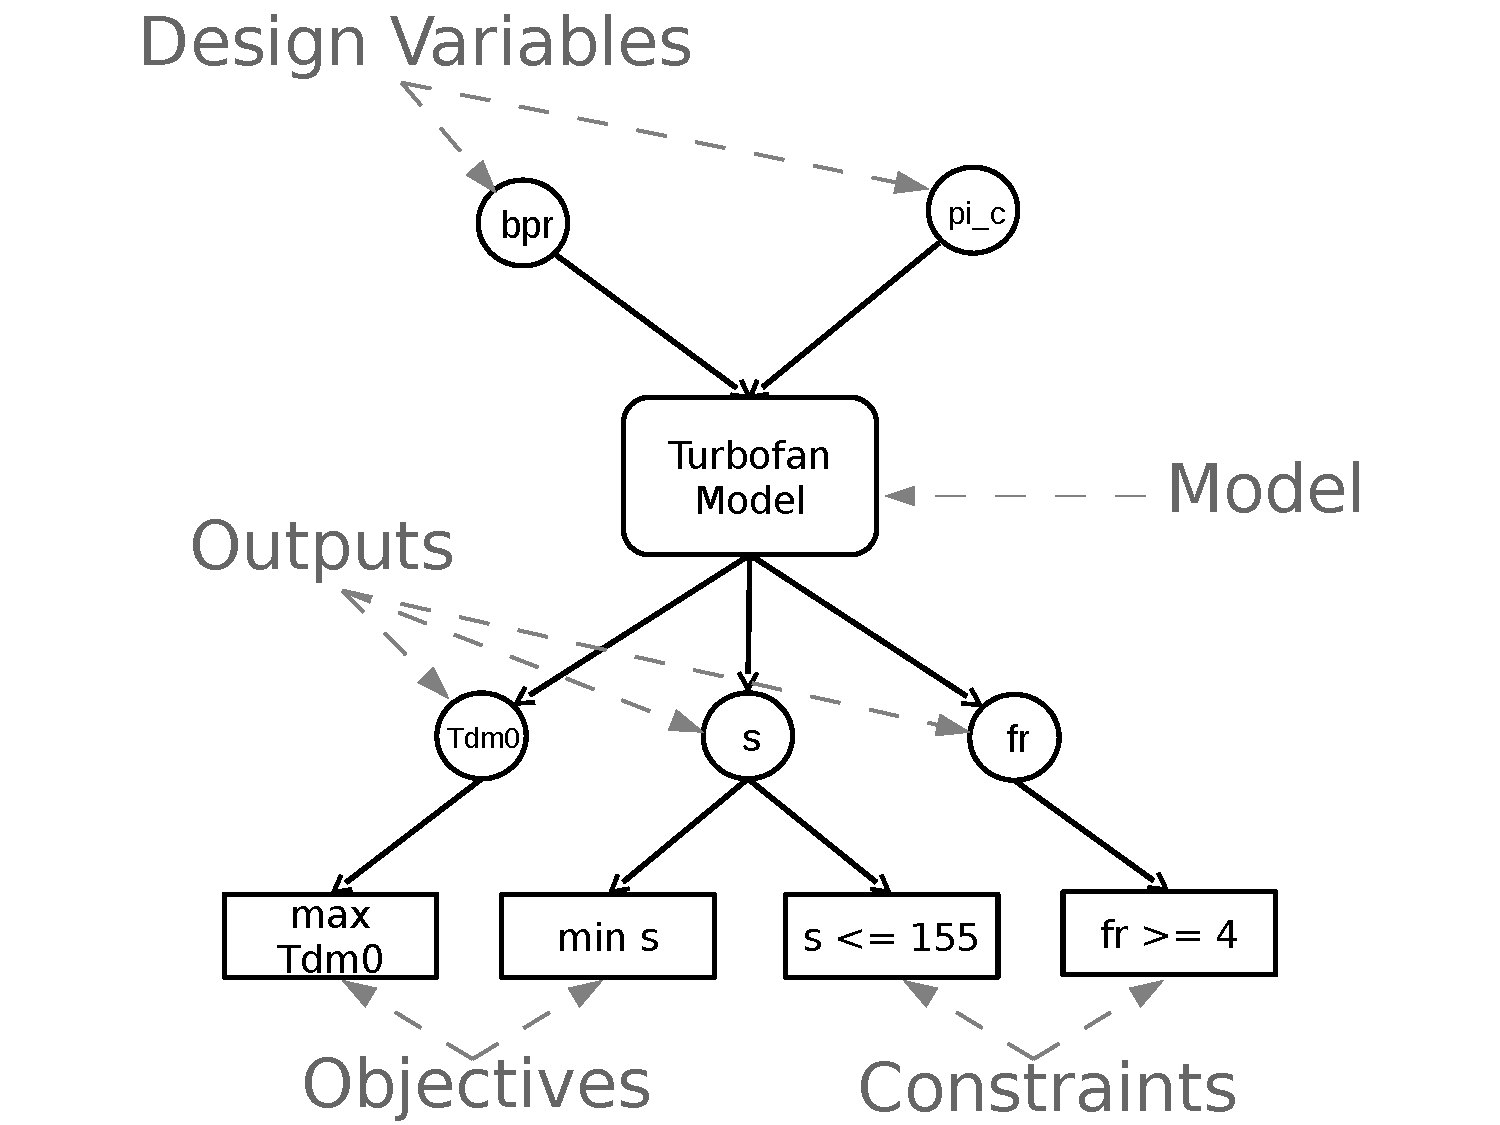
\includegraphics[width=\textwidth]{testcases-Turbofan-annoted}
\end{minipage}}

\caption{Turbofan problem.}
\label{turbofan}

\end{figure}

Let's now see in more details the roles of each of these fives entities: \emph{model}, \emph{variable}, \emph{output}, \emph{constraint} and \emph{objective}.

\subsubsection*{Models.}

In the most general case, a \emph{model} can be seen as a black box which takes input values (which can be \emph{design variables} or \emph{output variables}) and produces output values. A \emph{model} represents a technical knowledge of the relations between different parts of a problem and can be as simple as a linear function or a much more complex algorithm requiring several hours of calculation. Often some properties are known (or can be deduced) about a model and specialized optimization techniques can exploit this information.
In our Turbofan example, a \emph{model} entity is the $Turbofan$ function which calculate the three outputs using the values of $bpr$ and $pi\_c$.

\subsubsection*{Design Variables.}

These are the inputs of the problem and can be adjusted freely (within their defining boundaries). The goal is to find the set(s) of values for these variables that maximize the objectives while satisfying the constraints.
\emph{Design variables} are used by \emph{models} to calculate their outputs and by constraints and objectives to calculate their current value. A \emph{design variable} can be shared among several \emph{models}, objectives and constraints.
Keeping with our example, $bpr$ and $pi\_c$ are the two \emph{design variables} of our optimization problem.

\subsubsection*{Output Variables.}

These values are produced by a \emph{model}, and consequently cannot be changed freely.
As for the \emph{design variables}, the \emph{output variables} are used by \emph{models} to calculate their outputs and by constraints and objectives to calculate their current value.
In our example, $Tdm0$, $s$ and $fr$ are \emph{output variables} produced by the $Turbofan$ model.

\subsubsection*{Constraints.}

These are strict restrictions on some parts of the problem, represented as functional constraints defined by equalities and/or inequalities. These can be the expression of a physical constraint, or a requirement concerning the problem.
Regarding the Turbofan, the two \emph{constraints} are $s <= 155$ and $fr >=4$.

\subsubsection*{Objectives.}

The goals to be optimized. In the general case, different objectives are often contradictory.
The two  \emph{objectives} of the Turbofan problems are to maximize $Tdm0$ and to minimize $s$.

%Constraints and objectives are usually regrouped under the more general term of optimization criteria. 

%TODO what about the fact that constraints are more "important" (critical) than objectives and that objectives are all equivalent

\paragraph*{}
An interesting and important point is that both models, constraints and objectives involve computation. Often the most heavyweight calculus is encapsulated inside a model and the calculi concerning criteria tend to be simple equations, but this is neither an absolute requirement nor a discriminating characteristic.

The NDMO modeling aims to provide the most complete and natural representation of the problem. This modeling preserves the relations between the domain entities and is completely independent of the solving process. 
Since we now have a way to model optimization problems as graphs of entities, we now present the multi-agent algorithm proposed to solve them.

\section{From an Optimization Problem to a Multi-Agent System}

Based on the NDMO modeling in section \ref{modeling}, we propose a multi-agent system where each domain entity is associated with an agent. Thus the multi-agent system is the representation of the problem to be solved with the links and communication between agents reflecting the natural structure of the problem. It is worth underlining the fact that this transformation (\textit{i.e.} the agentification) can be completely automatic as it is fully derived from the expression of the problem.

The solving process - constituted by the collective behavior of the agents - basically relies, on change-value requests sent by the criteria agents resulting in cooperatively decided adjustments done by the \emph{design variables} and on new values computed by the models resulting on the satisfaction or dissatisfaction of the criteria agents. 
In the same way we presented the different elements of NDMO, we now detail the behaviors of our five agent types: \emph{model}, \emph{variable}, \emph{output}, \emph{constraint} and \emph{objective} agents.
A summary of the basic principles of each agent type is given in Algorithm \ref{agent_algo}.

\subsubsection*{Model Agent.}

A \emph{model agent} takes charge of a model of the problem. It interacts with the agents handling its inputs (which can be \emph{variable} or \emph{output agents}) and the \emph{output agents} handling its outputs. Its individual goal is to maintain the consistency between its inputs and its outputs. To this end, when it receives a message from one of its inputs informing it of a value change, a \emph{model agent} recalculates the outputs values of its model and informs its\emph{output agents} of their new value. On the other part, when a \emph{model agent} receives a message from one of its \emph{output agents} it translates and transmits the request to its inputs. 

To find the input values corresponding to a specific desired output value, the \emph{model agent} uses an external optimizer. This optimizer is provided by the engineer based on expert domain-dependent knowledge regarding the structure of the model itself.
It is important to underline that the optimizer is used only to solve the local problem of the \emph{model agent}, and is  not used to solve the problem globally.


%\begin{algorithm}
%\caption{Behavior of a Model Agent}
%\begin{algorithmic}
%\While{running}
%	\State Receive Messages
%	\If{received new informs}
%        \State recalculate outputs
%        \State inform output agents
%    \EndIf      
%	\If{received new requests}
%       \State  use optimizer to find adequate inputs
%        \State propagate requests to input agents
%    \EndIf
%\EndWhile
%\end{algorithmic}
%\end{algorithm}

\subsubsection*{Variable Agent.}

This agent represents a \emph{design variable} of the problem. Its individual goal is to find a value which is the best equilibrium among all the requests it can receive (from models and criteria for which it is an input). The agents using the variable as input can send to it request asking to change its value. When changing value, the agent informs all agents linked to it of its new value. 

%\begin{algorithm}
%\caption{Behavior of a Variable Agent}
%\begin{algorithmic}
%\While{running}
%	\State Receive Messages  
%	\If{received new requests}
%       \State select most important
%       \State adjust value
%       \State inform related agents
%    \EndIf
%\EndWhile
%\end{algorithmic}
%\end{algorithm}

To find its new value, the \emph{variable agent} uses an exploration strategy based on \emph{Adaptive Value Trackers} (AVT)\cite{Lemouzy_2011}. The AVT can be seen as an adaptation of dichotomous search for dynamic values. The main idea is to change value according to the direction which is requested and the direction of the past requests. While the value varies in the same direction, the variation delta is increased so the value varies more and more. As soon as the requested variation changes, it means that the variable went past the good value, so the variation delta is reduced.

%While changing value based not on the value requested but on the direction can seem paradoxical, it must be recalled that, since no agent has a global view of the system, the requests made by the agents is often approximate, so the agents need to iterate many times. If the search space in large, the system could take time to converge towards the solution. By using a near-dichotomous strategy, we greatly accelerate this convergence.

This capability to take into account a changing solution allows the \emph{variable agent} to continuously search for an unknown dynamic target value. This capability is also a requirement for the system to be able to adapt to changes made by the engineer during the solving process.

\subsubsection*{Output Agent.}
The \emph{output agent} takes charge of an output of a model. \emph{Output agent} and \emph{variable agents} have similar roles, except \emph{output agents} cannot directly change their value. Instead they send a request to the \emph{model agent} they depend on. In this regard, the \emph{output agent} act as a filter for the \emph{model agent} it depends on, selecting among the different requests the ones it then transmits.

%\begin{algorithm}
%\caption{Behavior of an Output Agent}
%\begin{algorithmic}
%\While{running}
%	\State Receive Messages
%	\If{received new informs}
%        \State update its value
%        \State inform related agents
%    \EndIf      
%	\If{received new requests}
%       \State  select most important
%        \State transmit selected request to model agent
%    \EndIf
%\EndWhile
%\end{algorithmic}
%\end{algorithm}

As we will see in the next section, the \emph{output agent} is distinct from the \emph{variable agent} in the way that it can be involved in cycles. A cycle is a situation of interdependent models (that is, models which depend of each other to calculate their outputs).

%We describe in the next section the main difficulties when solving an optimization problem including interdependencies, and how can an \emph{output agent} detect and handle them.

\subsubsection*{Constraint Agent.}
 \emph{The constraint agent} has the responsibility for handling a constraint of the problem. When receiving a message from one of its inputs, the agent recalculates its constraint and checks its satisfaction. If the constraint is not satisfied, the agent sends \emph{change value} requests to its inputs.

%\begin{algorithm}
%\caption{Behavior of a Constraint/Objective Agent}
%\begin{algorithmic}
%\While{running}
%	\State Receive Messages
%	\If{received new informs}
%        \State update its value
%        \State use optimizer to find adequate inputs
%        \State send new requests to input agents
%    \EndIf      
%\EndWhile
%\end{algorithmic}
%\end{algorithm}

It should be noted that, to estimate the input values required to satisfy the constraint on its computed value, this agent employs the same technique as the \emph{model agent} (\textit{i.e.} an external optimizer).

\subsubsection*{Objective Agent.}
The  \emph{objective agent} is in charge of an objective of the problem. This agent sends requests to its inputs aiming to improve its objective, and recalculates the objective when receiving  \emph{value changed} messages from its inputs.

This agent uses an external optimizer to estimate input values which would improve the objective, as the model and constraint agents.

\paragraph*{}
The most important point is that each agent only has a local strategy. No agent is in charge of the optimization of the system as a whole, or even of a subset of the other agents. Contrary to the classical MDO methods presented earlier, the solving of the problem is not directed by a predefined methodology, but by the structure of the problem itself. The emerging global strategy is unique and adapted to the problem.

\begin{algorithm}
\caption{Agents Behaviors}
\label{agent_algo}
\begin{algorithmic}[[TODO: correct algo formatting]]

\Procedure{Model Agent Behavior}{}
\Loop
	\State analyze received messages
	\If{received new information messages}
        \State recalculate outputs
        \State inform depending agents
    \EndIf      
	\If{received new requests}
       \State  use optimizer to find adequate inputs
        \State propagate requests to input agents
    \EndIf
\EndLoop
\EndProcedure
\\
\Procedure{Variable Agent Behavior}{}
\Loop
	\State analyze received messages
	\If{received new requests}
       \State select most important
       \State adjust value
       \State inform depending agents
    \EndIf
\EndLoop
\EndProcedure
\\
\Procedure{Output Agent Behavior}{}
\Loop
	\State analyze received messages
	\If{received new information messages}
        \State update its value
        \State inform depending agents
    \EndIf      
	\If{received new requests}
       \State  select most important
        \State transmit selected request to model agent
    \EndIf
\EndLoop
\EndProcedure
\\
\Procedure{Constraint/ Objective Agent Behavior}{}
\Loop
	\State analyze received messages
	\If{received new information messages}
        \State update its value
        \State use optimizer to find adequate inputs
        \State send new requests to variable/output agents
    \EndIf      
\EndLoop
\EndProcedure
\end{algorithmic}
\end{algorithm}




\chapter{Simulation Rules}

\chapter{Solving Rules}

\chapter{Implementation}

\section{MAY Architecture}

To implement the MAS, we used the Make Agents Yourself (MAY) framework. MAY is a component-based framework which automatically generate an implementation of an agent architecture from a given description.

[[PROVIDE SOME REF -> ASK VICTOR]]

The Adelfe methodology proposes an abstract agent architecture (represented in \fig{[[TODO]]}), which we translated into the MAY architecture description language, SpeADL. [[As our agents only act and communicate using message-passing, we could make some simplification concerning the modeling of the communication and action capabilities.]]
All our agents use the same AMAS architecture. They are differentiated by specific implementations of the components. For example, \emph{Model} and \emph{Variable} agents will have different implementations of the \emph{Behavior} component.

For the sake of clarity, the agent architecture is separated in three views: the \emph{behavior}, \emph{communication} and \emph{monitoring} views.

\subsection{Behavior}

The \emph{behavior} view (\figurename{} \ref{Arch-behavior}) contains the components related to the behavior of the agent. 

\begin{figure}
\centering
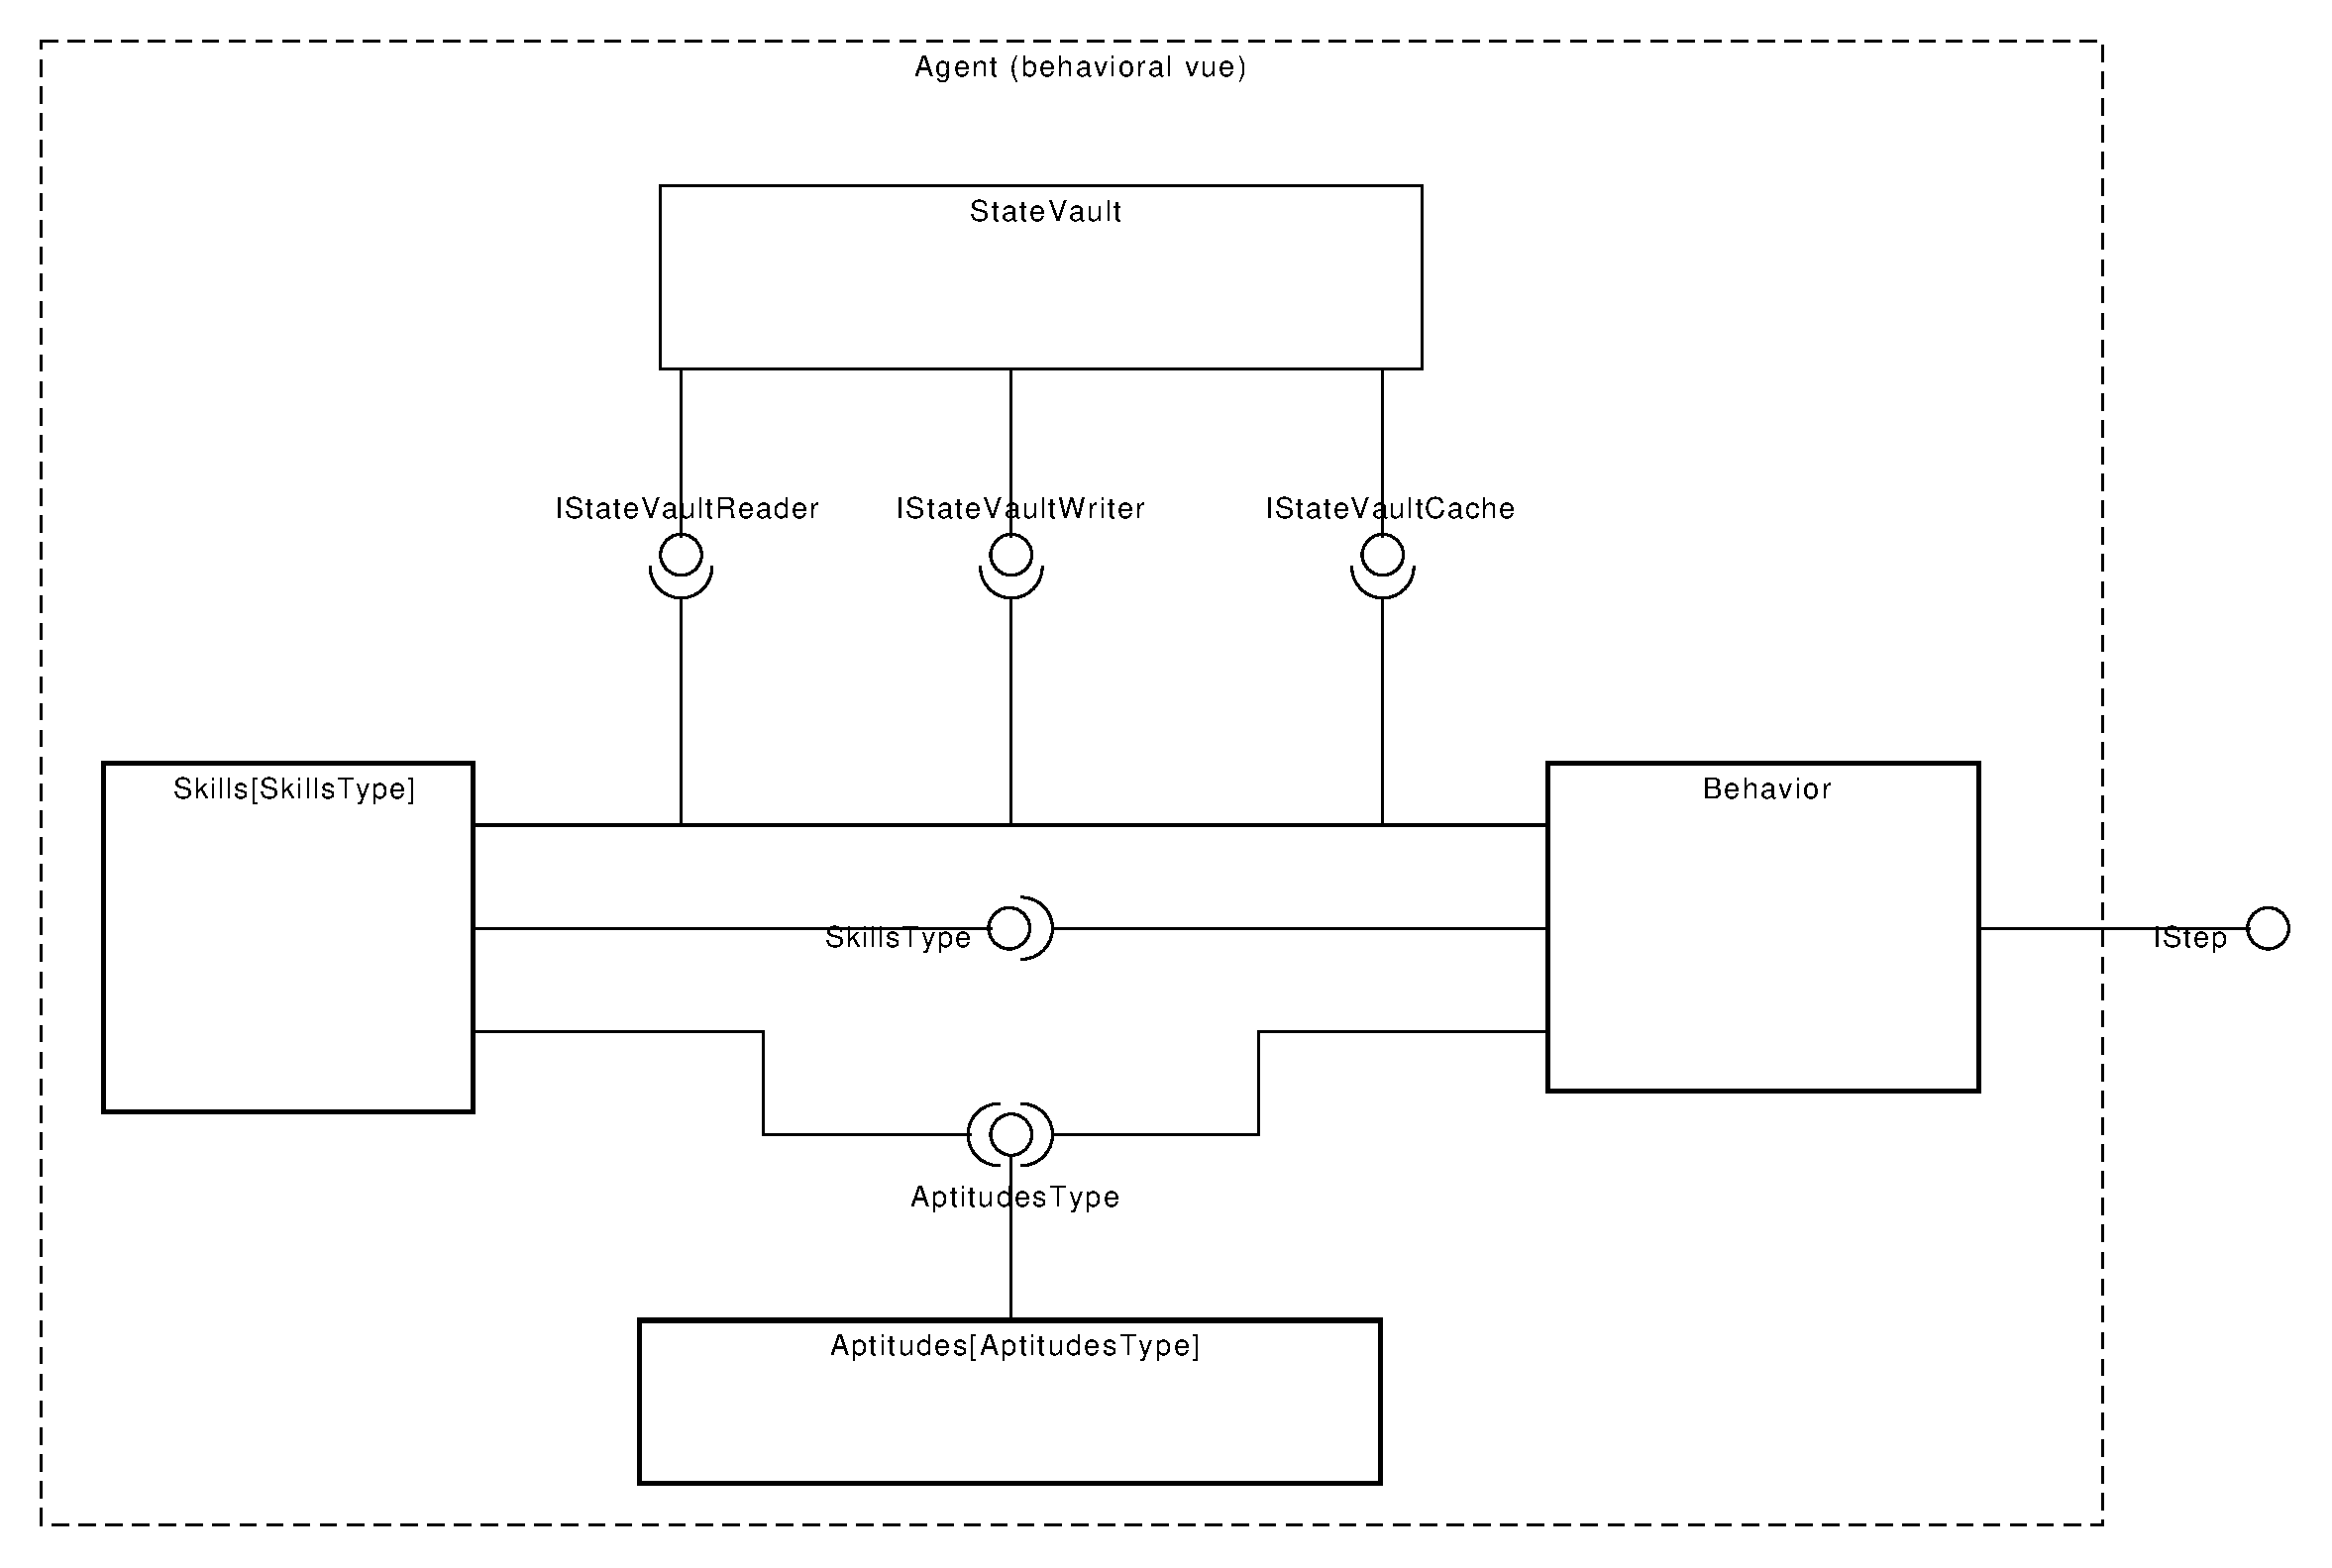
\includegraphics[width=0.6\paperwidth]{ID4CS_Speadl_behav}
\caption{Agent Architecture - Behavior view.}
\label{Arch-behavior}
\end{figure}

The \emph{Behavior} component contains the rules which dictate the behavior of the agent. This component can be seen as the [[chef d'orchestre]] of the architecture. This component exposes to the outside of the environment the \emph{Step} port, which is used to make the agent execute a step. During a step the \emph{Behavior} component executes the agent rules. These rules will in return make use of the others components of the agent.

[[DIRE QUE LES RULES ONT ETE PRESENTEES DANS UN CHAPITRE PRECEDENT]]

The \emph{State Vault} contains the state of the agent. It is used by the components which need to save and read some state variables. Centralizing all the states variables into one component provides several benefits. First it is easier to save and restore the state of the agent, as we just need to save the content of the vault. It is also simple to share some data between components, as long as these components have access to the vault. And it is easy to provide a view of the agent state by just reading the State Vault.
This approach has however several drawbacks. It adds some boilerplate code when writing code using the agent state, as we need to explicitly read the value from the vault (and possibly store it to the vault if modified). It make more difficult to track side-effects, as it is not obvious to know which component uses which value. At last there is no way to strictly enforce that components only use the State Vault for storing state values, as neither Java nor MAY can provide such guarantee.

The \emph{Skills} component contains the skills of the agents. Skills are [[skill definition]]. Each agent type has its own skills set, and skills can require to read and modify the agent state (thus the link between this component and the \emph{State Vault}).
Some skills are used directly from the \emph{Behavior} rules but some skills can also be used by others skills.
Some examples of skills are: for a \emph{Variable agent}, the capability to change its value based on the requests it received and its old value. For a model agent, the capability to translate a request it received to change one of its outputs into a set of requests to send to its inputs.

[[PARLER DU FAIT QUE LES SKILLS ONT LEUR PROPRE ARCHITECTURE ??]]

The \emph{Aptitudes} component contains the aptitudes accessible to the agents. Aptitudes are [[Aptitude definition]]. Unlike skills, aptitudes are general capabilities which do not rely on the state of the agent. Consequently, all agent types have access to the same aptitudes, and there is only one implementation of the \emph{Aptitudes} component.
Some aptitudes are used directly from the \emph{Behavior} rules but some aptitudes can also be used by skills or others aptitudes.
Some examples of aptitudes are: ordering a set of requests from the most to the least important. Make some manipulations on the exchanged values (adding, calculate the norm etc.).

\subsection{Communication}

The \emph{communication} view (\figurename{} \ref{Arch-comm}) presents the components related to the communication capabilities of the agent. 

\begin{figure}
\centering
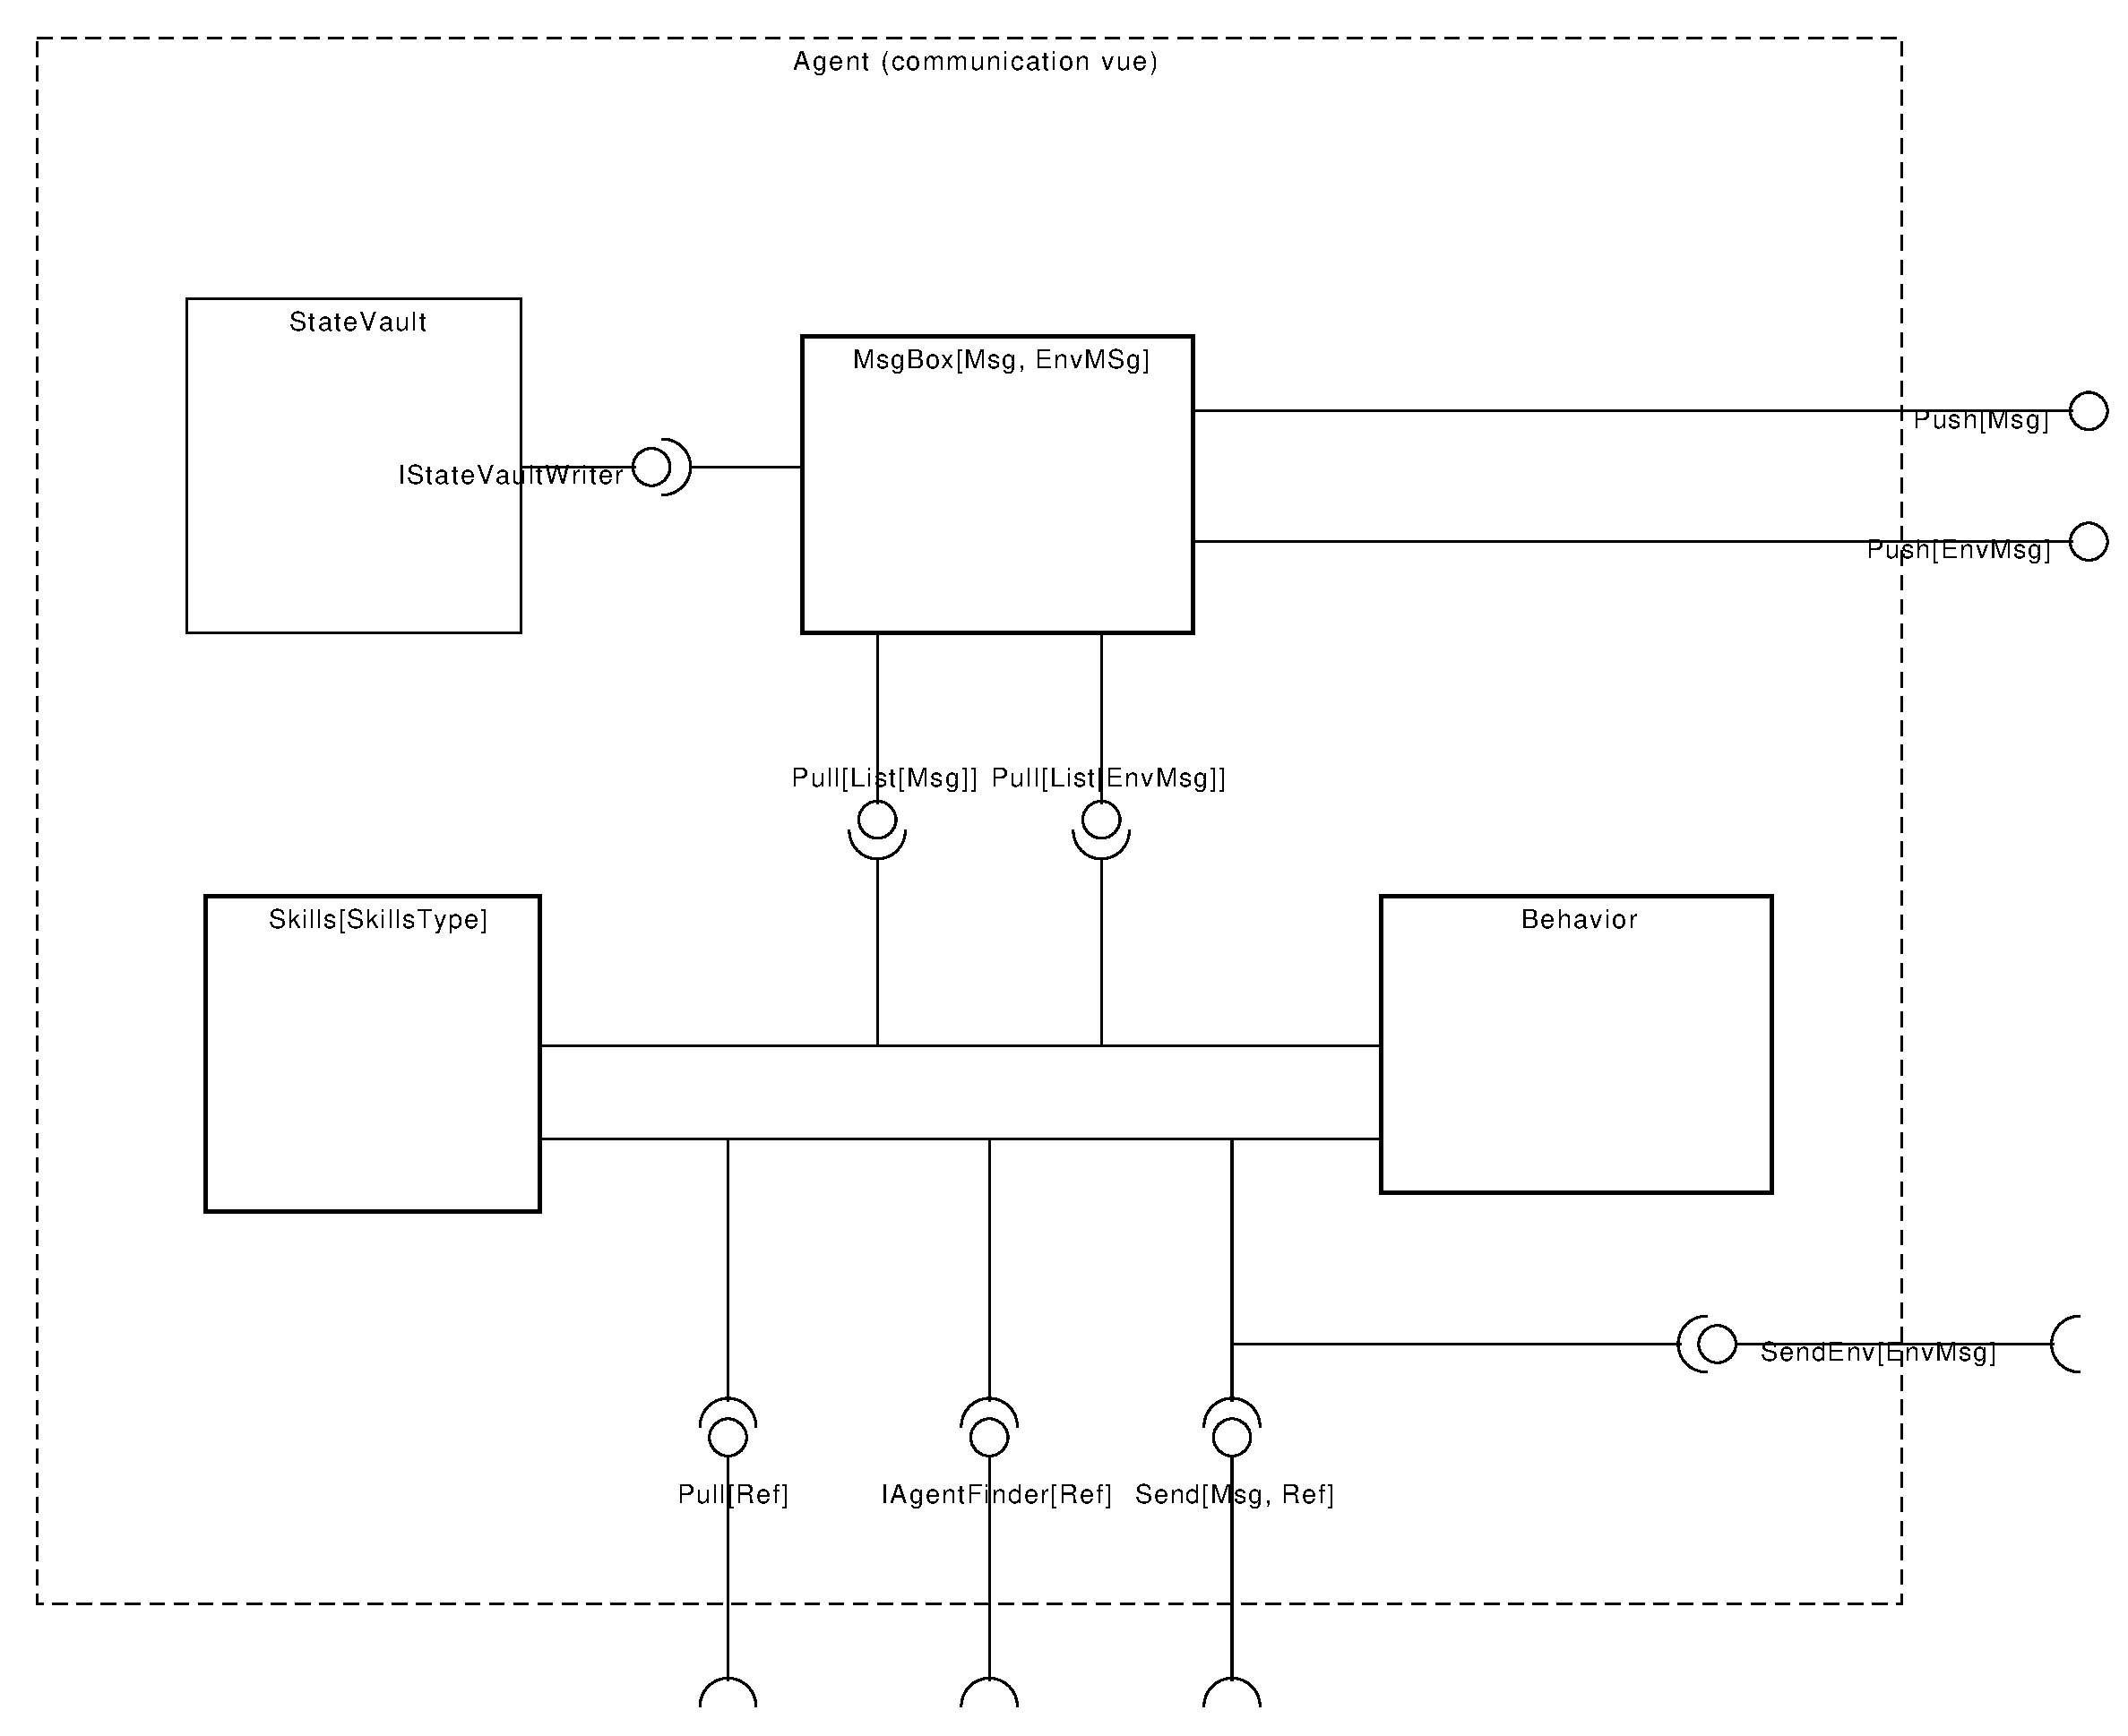
\includegraphics[width=0.6\paperwidth]{ID4CS_Speadl_comm}
\caption{Agent Architecture - Communication view.}
\label{Arch-comm}
\end{figure}

This view contains the new component \emph{Message Box}, which contains the messages sent to the agent. The \emph{Message Box} stores the messages into the \emph{State Vault} and provides a direct access to the \emph{Skills} and {Behavior} components.

This figure presents several ports which need to be provided from the environment to the agent. The environment must give an unique \emph{Reference} to the agent, which will be used by the others agent to communicate with it. The environment must also provides some ports to communicate with the others agents and outside of the system.
[[PARLER DE L'AGENT FINDER ??]]

\subsection{Monitoring}

The \emph{monitoring} view (\figurename{} \ref{Arch-monitor}) presents the components related to the monitoring of the agent. 

The new component introduced in this view is the \emph{Monitor}. The \emph{Monitor} provides to the environment to ports. The first port is used for external monitoring interfaces to subscribe to be informed of changes in the state of the agent. The second is used to provide informations concerning changes of a specific part of the agent. Thus, an external monitoring interface can subscribe to be notified when the state of the agent changed using the first port, and then use the second port to access to the specific informations it want to monitor.

In order to provide its capabilities, the monitor agent need to be informed by the \emph{Behavior} component before and after each step, to read and compare the monitored informations into the \emph{State Vault}.

\begin{figure}
\centering
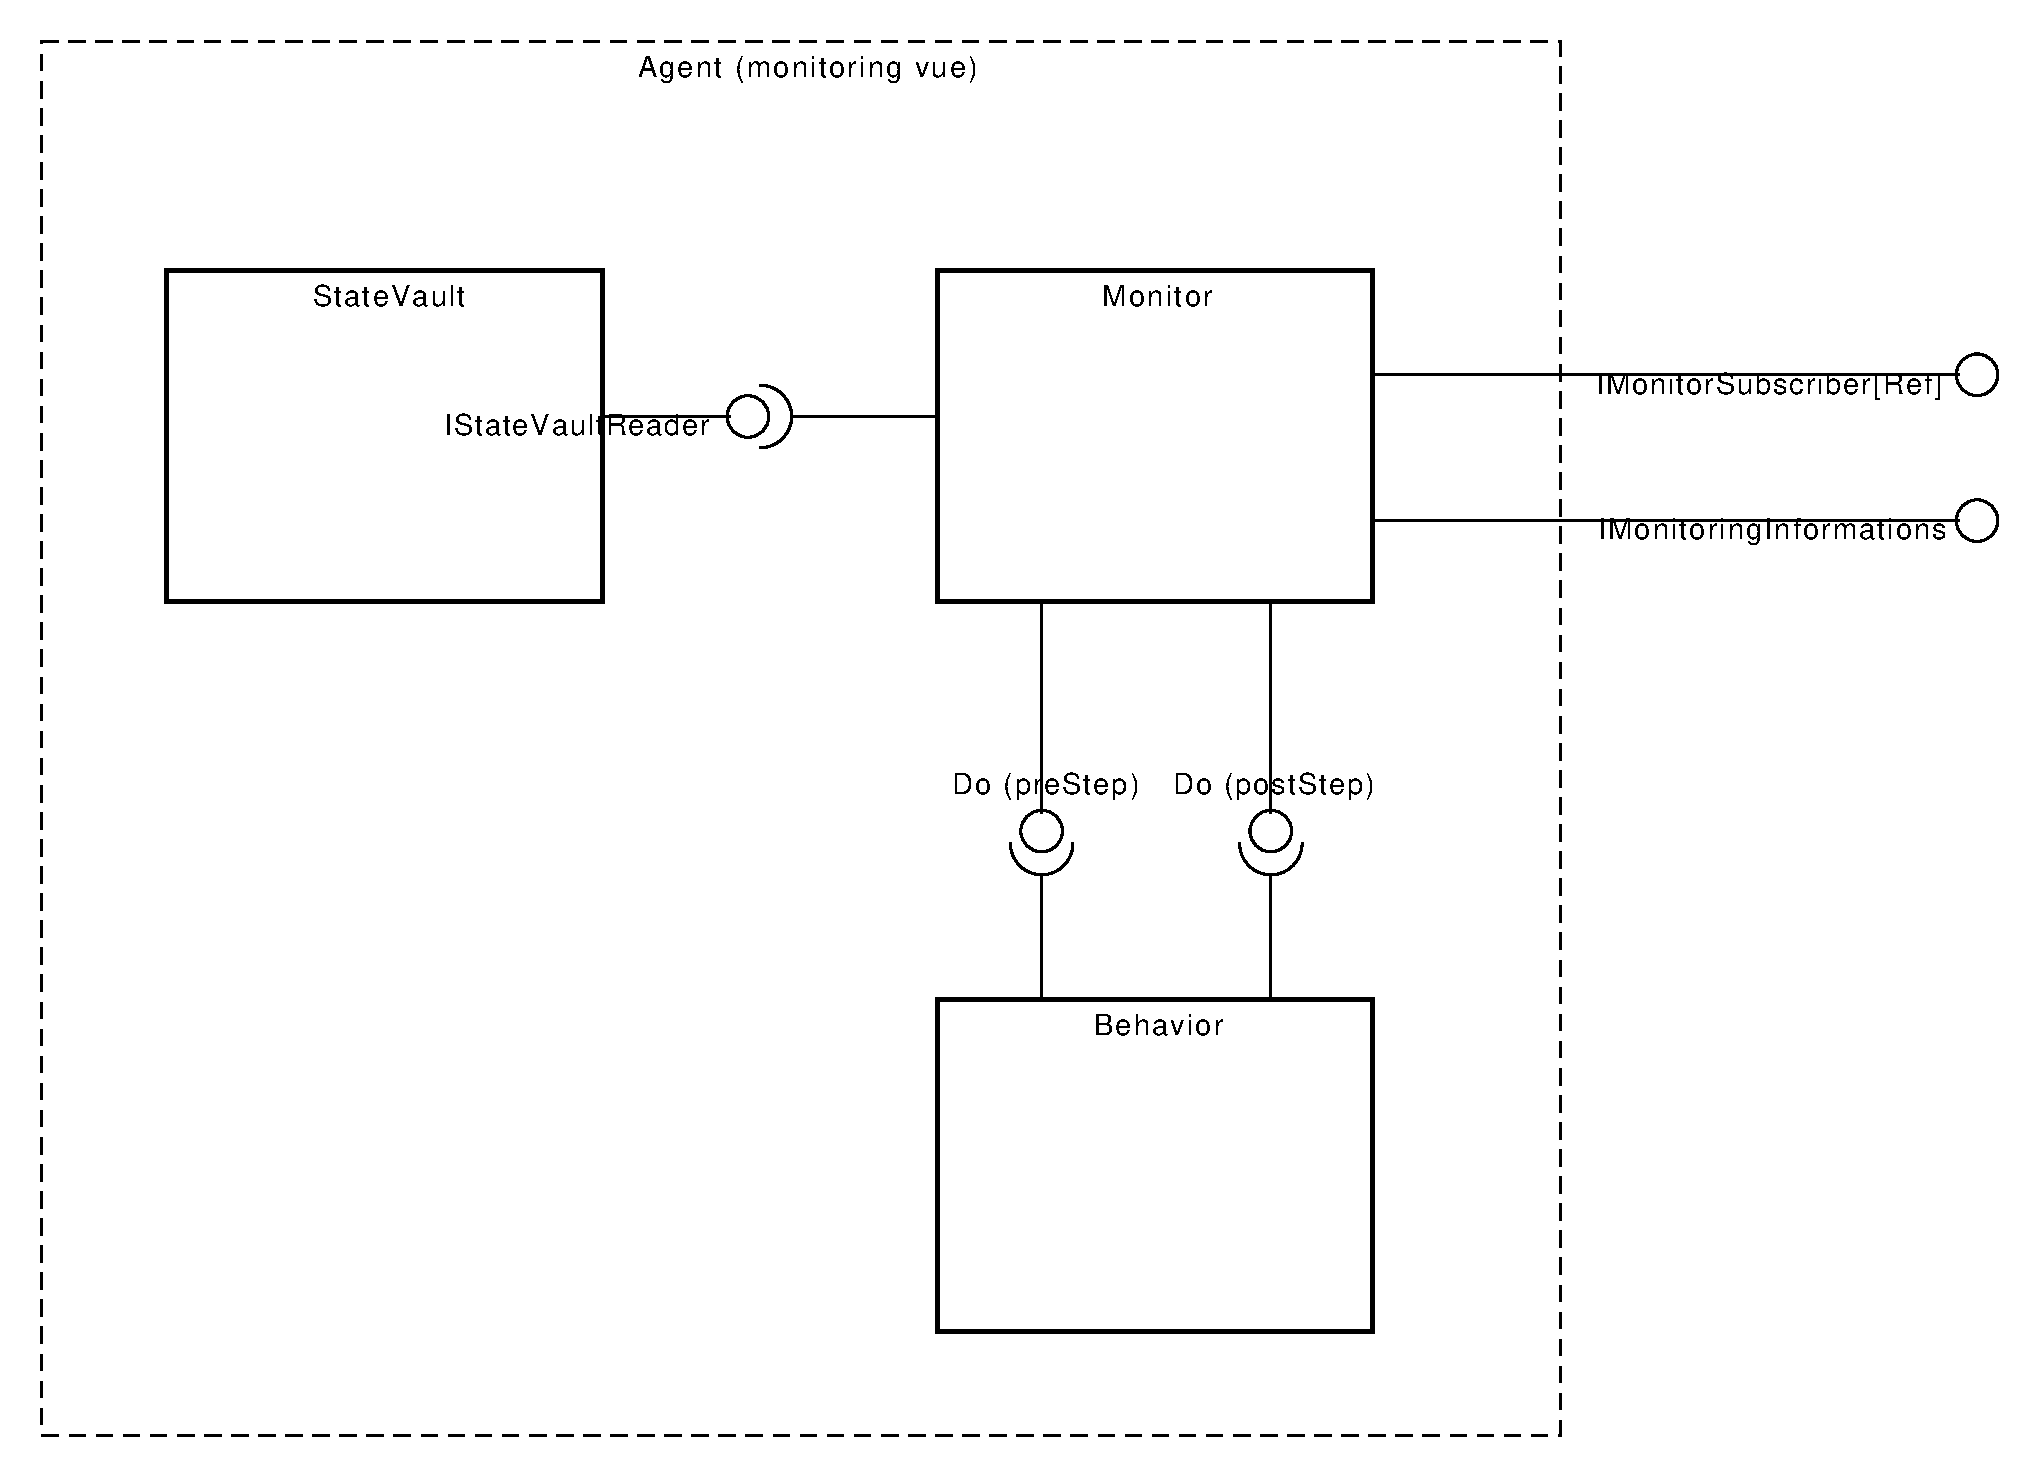
\includegraphics[width=0.6\paperwidth]{ID4CS_Speadl_monitoring}
\caption{Agent Architecture - Monitoring view.}
\label{Arch-monitor}
\end{figure}

\section{MAS Architecture}

\section{Integration into the prototype}

[[OSGI and EMF]]

\chapter{Analysis - Collective Solving Patterns}